%%%%%%%%%%%%%%%%%%%%%%%%%%%%%%%%%%%%%%%%%
% University/School Laboratory Report
% LaTeX Template
% Version 4.0 (March 21, 2022)
%
% This template originates from:
% https://www.LaTeXTemplates.com
%
% Authors:
% Vel (vel@latextemplates.com)
% Linux and Unix Users Group at Virginia Tech Wiki
%
% edited by:
% Johann Becker, Marc Ostner, Valentin Eder
%
% License:
% CC BY-NC-SA 4.0 (https://creativecommons.org/licenses/by-nc-sa/4.0/)
%
%%%%%%%%%%%%%%%%%%%%%%%%%%%%%%%%%%%%%%%%%

%----------------------------------------------------------------------------------------
%	PACKAGES AND DOCUMENT CONFIGURATIONS
%----------------------------------------------------------------------------------------
\documentclass[
	a4paper, % Paper size, specify a4paper (A4) or letterpaper (US letter)
	12pt, % Default font size, specify 10pt, 11pt or 12pt
]{CSUniSchoolLabReport}
\usepackage[ngerman]{babel}
\usepackage{siunitx}  
\usepackage{textcase}
\usepackage{booktabs}
\usepackage[utf8]{inputenc}
\usepackage{amsmath}
\usepackage{array}
\usepackage{enumitem} % für präzise Kontrolle über Listen
\usepackage{mhchem}
\usepackage{pdfpages}
\usepackage{float}
\usepackage{csquotes} % Recommended for biblatex with babel/polyglossia
\sisetup{locale = DE,  
separate-uncertainty,  
range-units = brackets,  
list-units = single,  
per-mode=symbol-or-fraction,
}  
\addbibresource{sample.bib} % Bibliography file (located in the same folder as the template)
\renewcommand{\thesection}{\Alph{section}}
\renewcommand{\thesubsection}{\thesection.\arabic{subsection}}
\renewcommand{\thesubsubsection}{\thesubsection.\arabic{subsubsection}}
\makeatletter
\renewcommand\paragraph{\@startsection{paragraph}{4}{\z@}%
  {-3.25ex \@plus -1ex \@minus -0.2ex}%
  {1.5ex \@plus 0.2ex}%
  {\normalfont\normalsize\bfseries}}
\makeatother
\renewcommand{\theparagraph}{\alph{paragraph})}
\newcommand{\micro}{\ensuremath{\mu}}
\newcommand{\pico}{p}
\newcommand{\milli}{m}
\newcommand{\nano}{n}
\newcommand{\RNum}[1]{\uppercase\expandafter{\romannumeral #1\relax}}%----------------------------------------------------------------------------------------
%	REPORT INFORMATION
%----------------------------------------------------------------------------------------
\setlength{\parindent}{0pt}

\title{Protokoll zum Praktikumsversuch Bipolartransistor in Elektronische Bauelemente} % Report title

\author{Johann \textsc{Becker} \and Valentin \textsc{Eder} \and Marc \textsc{Ostner}}
\date{\today} % Date of the report

%----------------------------------------------------------------------------------------

\begin{document}

\maketitle % Insert the title, author and date using the information specified above


\begin{center}
	\begin{tabular}{l r}
		Date Performed: & 20. Juni 2025 \\ % Date the experiment was performed
		
		Instructor: & Prof. Dr. Alexandru Negut % Instructor/supervisor
	\end{tabular}
\end{center}

% If you need to include an abstract, uncomment the lines below
%\begin{abstract}
%	Abstract text
%\end{abstract}

%----------------------------------------------------------------------------------------
%	OBJECTIVE
%----------------------------------------------------------------------------------------

\section{Einführung}
\subsection{Gegenstand des Versuchs}
In diesem Versuch sollen Eigenschaften und Anwendungen des Bipolartransistors BD137-16 untersucht werden.
\subsection{Notwendige Vorbereitungen}
\subsubsection{Versuchsablauf}
Die dynamische Messung der Transistorkennlinien erfolgt ähnlich zu der Messung von Diodenkennlinien.
\subsubsection{Datenblatt}
Der BD137-16 ist ein NPN Silizium Transistor. 
Der ``-16'' Anhang steht für die dynamische Stromverstärkung $\beta_{\RNum{3}}$, in diesem Fall 100\textasciitilde 250. 

\subsection{Fragen zum Verstärker}
Hier nicht ausgeführte Fragen finden sich im Anhang.
\paragraph{a) Welche Aufgabe hat der Kondensator $C_k$ und wie herum muss ein gepolter Elektrolytkondensator an dieser Stelle eingebaut werden?}
Der Koppelkondensator $C_k$ trennt den Gleichspannungsanteil vom Signal und lässt nur das Wechselspannungssignal durch.
Hierdurch kann ein Transistor Arbeitspunkt unabhängig von der Signalquelle $U_{sig}$ eingestellt werden. Als resultat bleibt der Großsignal Arbeitspunkt bestehen, während die Kleinsignaländerungen von $U_{sig}$ weiterhin bestehen bleiben. 



Ein gepolter Elektrolytkondensator muss so eingebaut werden, dass die positive Seite an die höhere Gleichspannung angeschlossen wird.


\paragraph{e) Auf welchen Wert sollte der ausgangsseitige Arbeitspunkt $U_{CE}$ eines Verstärkers in Emitterschaltung sinnvollerweise eingestellt werden? }

Der Arbeitspunkt sollte in der ``Safe Operation Area`` eingestellt werden, um die Verstärkung möglichst wenig zu Verzerren. Also sollte $U_{CE}$ überhablb des Sättigungsbereichs liegen, aber unter der maximalen ableitbaren Leistung. 
Um eine maximale Verstärkungsamplitude zu gewährleisten, sollte $U_{CE\,AP}$ im Mittel dieser beiden Spannungen $U_{CE\,\text{Sättigung}}$ und $U_{CE\,\text{PMax}}$ liegen.




% B.
\section{Versuchsdurchführung}
% B.1.
\subsection{Kennlinien }
% B.1.1.
\subsubsection{Ausgangskennlinienfeld}

\begin{figure}[H]
	\centering
	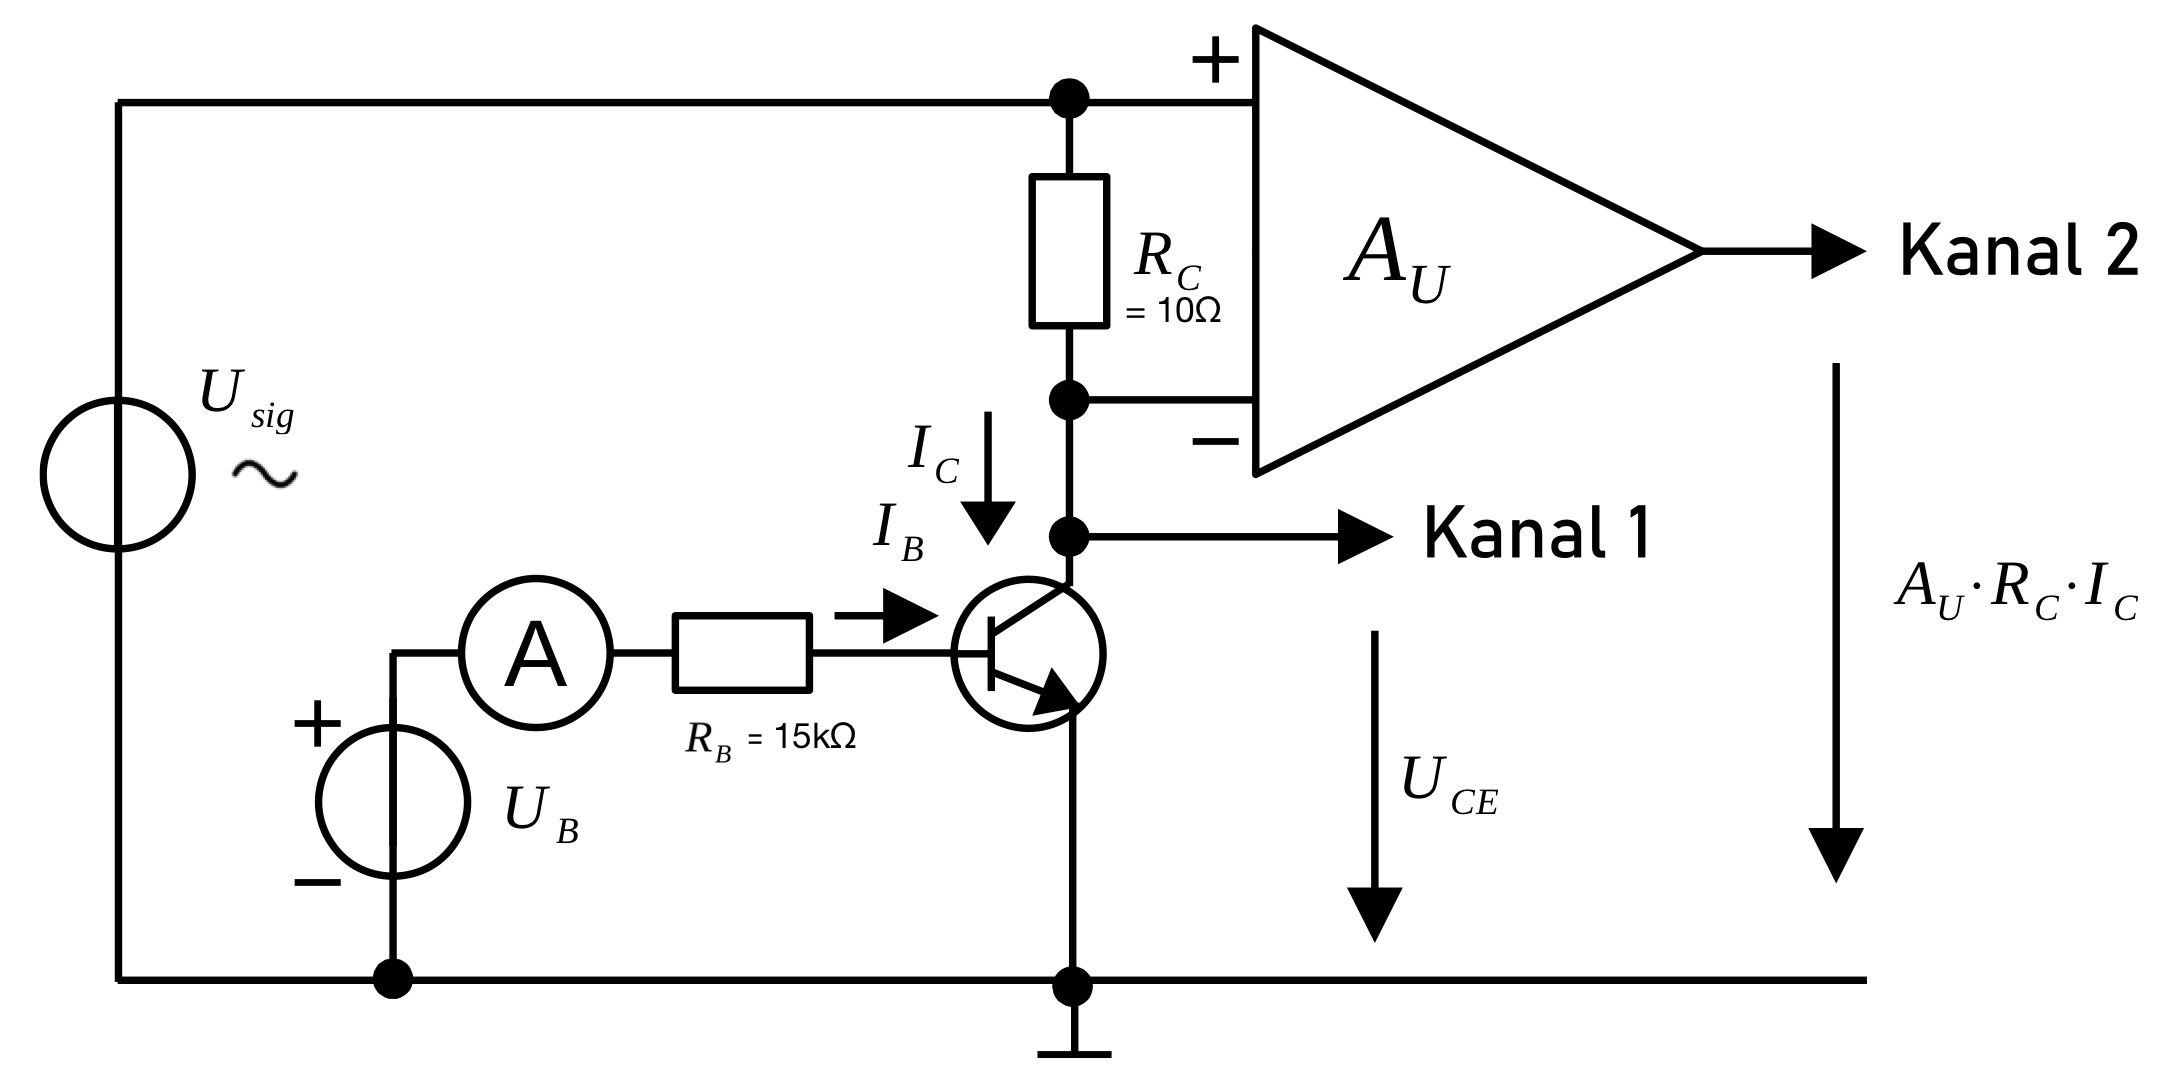
\includegraphics[width=0.7\textwidth]{Figures/MessschaltungAusgangskennlinienfeld.png}
	\caption{Messschaltung zur Aufnahme des Ausgangskennlinienfeldes des BD137-16.}
	\label{fig:MessschaltungAusgangskennlinienfeld}
\end{figure}
\begin{figure}[H]
	\centering
	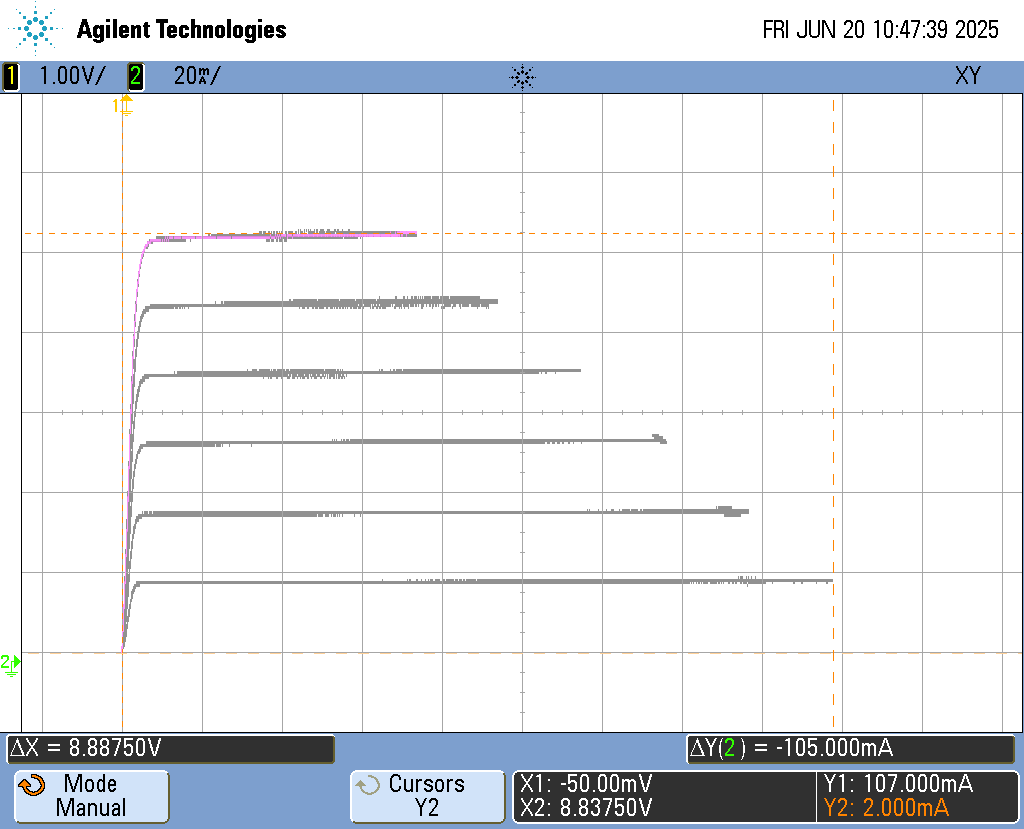
\includegraphics[width=0.8\textwidth]{Figures/Ausgangskennlinienfeld.png}
	\caption{Gemessenes Ausgangskennlinienfeld.}
	\label{fig:Ausgangskennlinienfeld}
\end{figure}

Das Ausgangskennlinienfeld wird jeweils in Schritten von $\Delta I_B = \SI{100}{\micro\ampere}$ aufgenommen.

% B.1.2.
\subsubsection{Eingangskennlinie}
\begin{figure}[H]
	\centering
	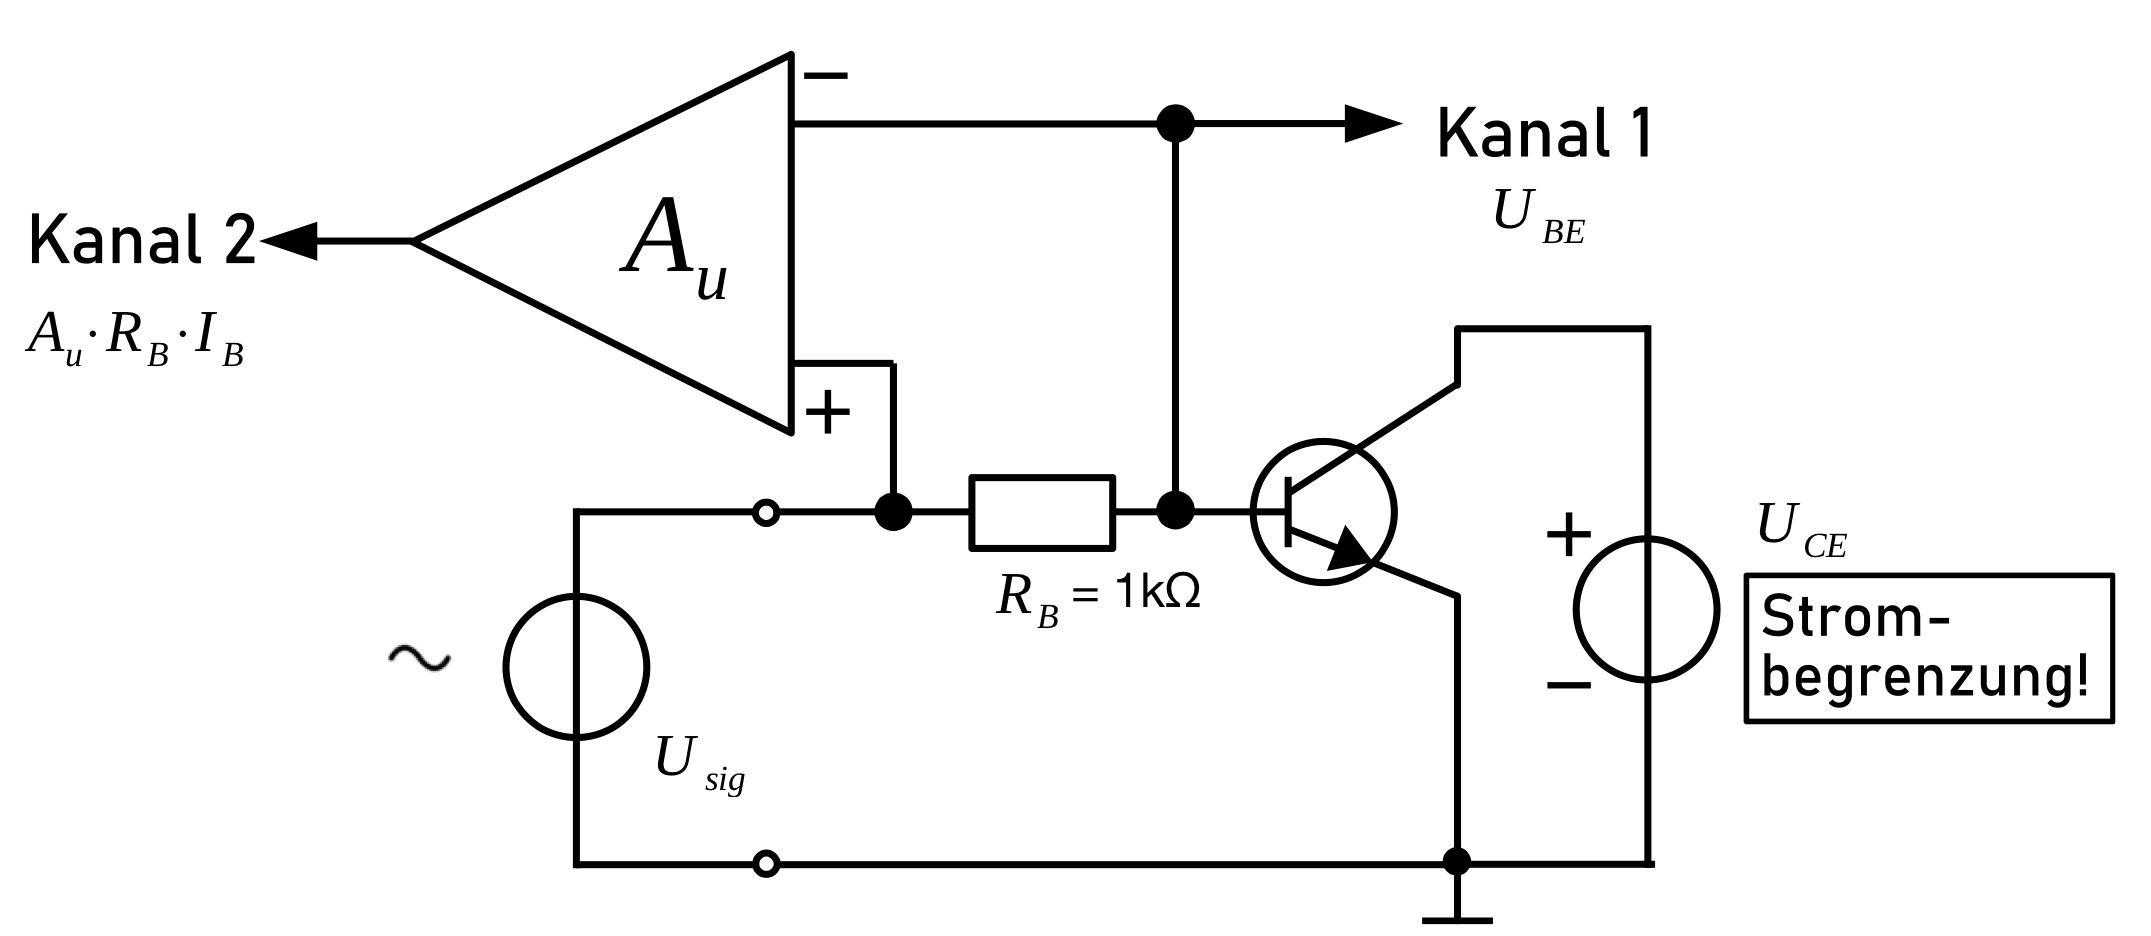
\includegraphics[width=0.8\textwidth]{Figures/MessschaltungEingangskennlinie.png}
	\caption{Messschaltung zur Aufnahme der Eingangskennlinie des BD137-16.}
	\label{fig:MessschaltungEingangskennlinie}
\end{figure}
\begin{figure}[H]
	\centering
	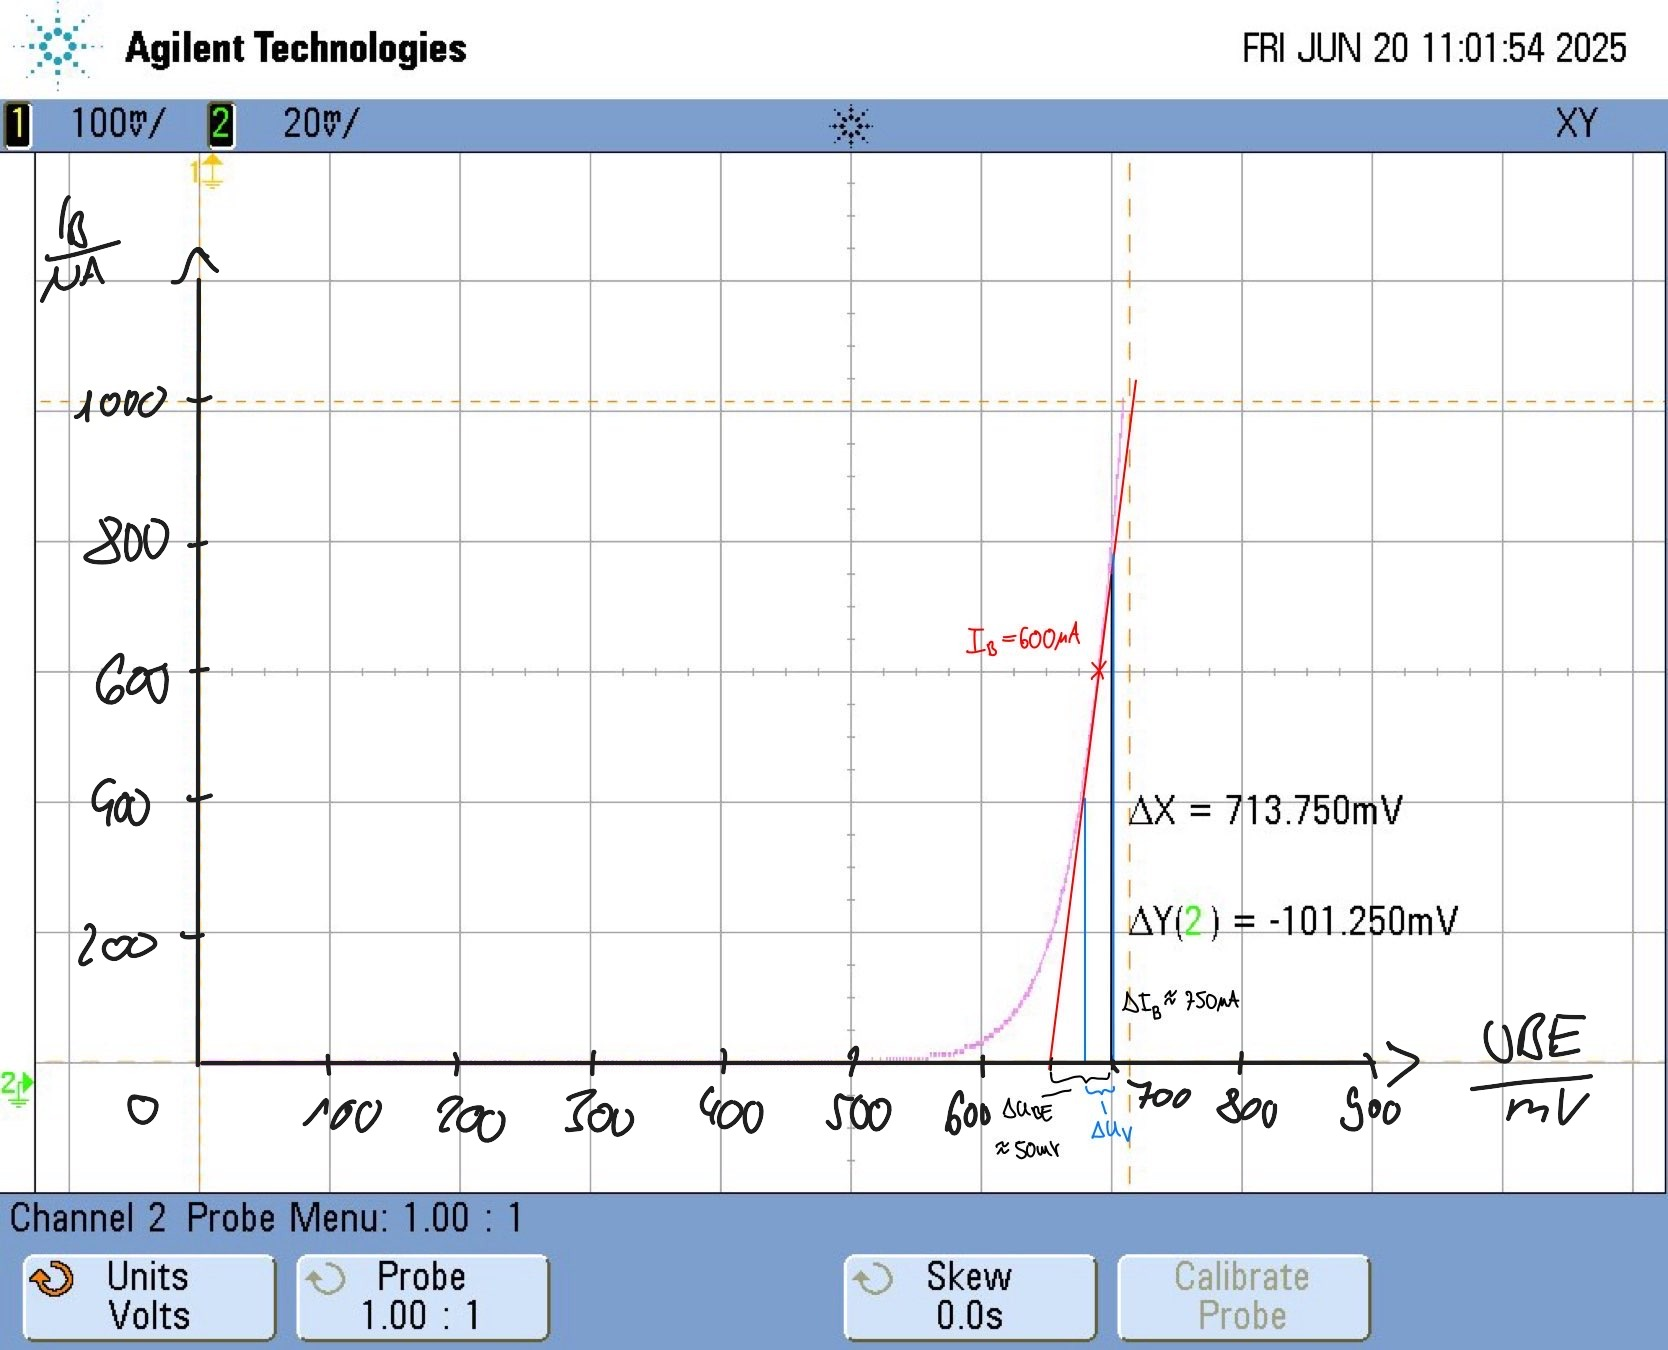
\includegraphics[width=0.8\textwidth]{Figures/Eingangskennlinie.jpg}
	\caption{Bestimmung von $\Delta U_{BE}$ und $\Delta I_B$}
	\label{fig:Eingangskennlinie}
\end{figure}



Für diese Messung ist wichtig, die Spannungsquelle direkt am Kollektor und Emitter anzulegen, um die Spannung so Konstant wie möglich zu halten.
Um eine Zerstörung des Transistors bei fehlerhaften Versuchsdurchführung zu verhindern, muss die Strombegrenzung der Spannungsquelle auf \SI{250}{\milli\ampere} eingestellt werden. 
Der Basisstrom wird über den Spannungsabfall an $R_B$ bestimmt.

% B.1.3.
\subsubsection{Temperaturverhalten}
\begin{figure}[H]
	\centering
	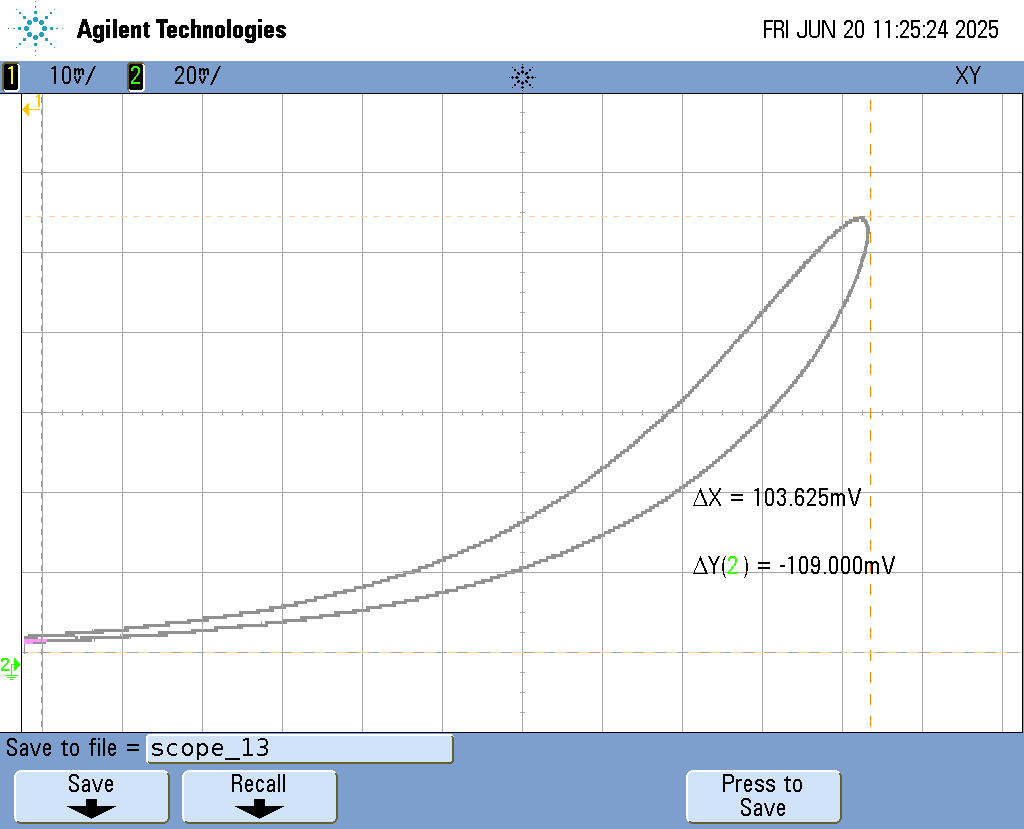
\includegraphics[width=0.8\textwidth]{Figures/TemperaturHysterese8V0.1hznah.png}
	\caption{Hysterese des BD137-16 bei $U_{CE} = 8\,\mathrm{V}$ und $f = 0{,}1\,\mathrm{Hz}$.}
	\label{fig:8VTemperaturHysterese0.1hznah}
\end{figure}
\begin{figure}[H]
	\centering
	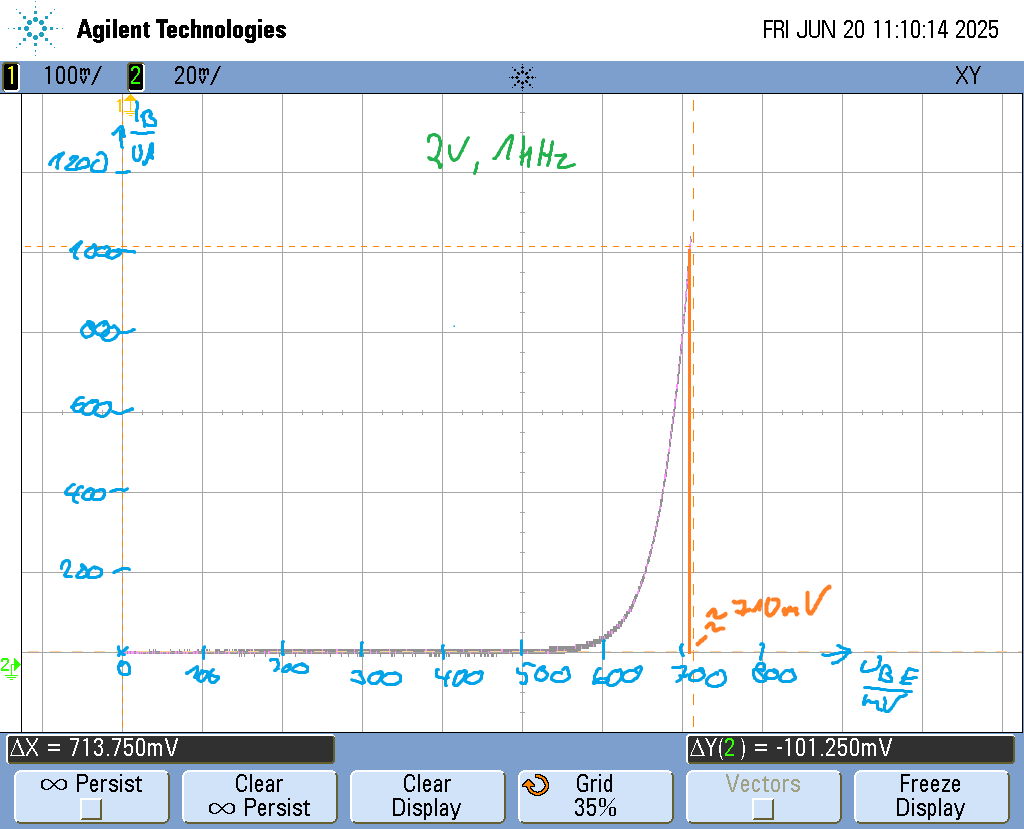
\includegraphics[width=0.8\textwidth]{Figures/temp2v1khz.png}
	\caption{Eingangskennlinie bei $\SI{2}{\volt}$ und $\SI{1}{\kilo\hertz}$.}
	\label{fig:2V1eingang}
\end{figure}
\begin{figure}[H]
	\centering
	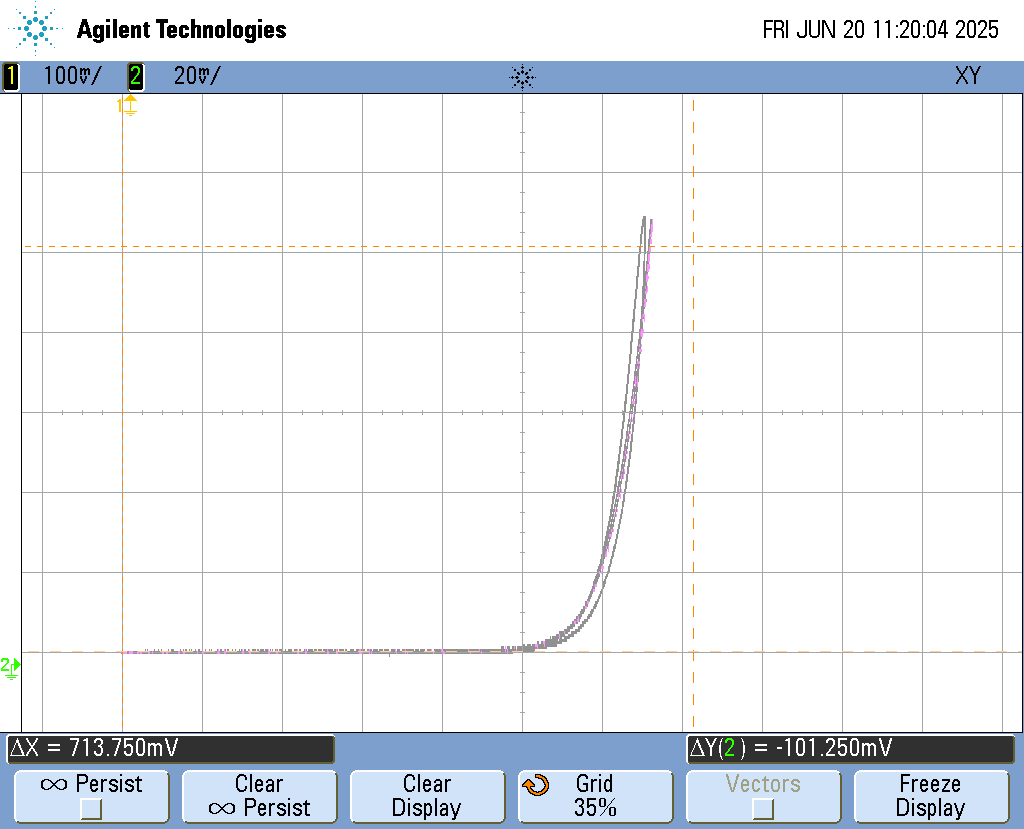
\includegraphics[width=0.8\textwidth]{Figures/8V1khz0.1hzzusammentemp.png}
	\caption{Temperaturverhalten bei $U_{CE} = \SI{8}{\volt}$ und $f = 0{,}1\,\mathrm{Hz}$ sowie $f = \SI{1}{\kilo\hertz}$.}
	\label{fig:8V1khz0.1hzzusammentemp}
\end{figure}

% B.1.4.
\subsubsection{Übertragungskennlinie}
\begin{figure}[H]
	\centering
	\includegraphics[width=0.8\textwidth]{Figures/MessschaltungÜbertragungskennlinie.png}
	\caption{Messschaltung zur Aufnahme der Übertragungskennlinie.}
	\label{fig:MessschaltungÜbertragungskennlinie}
\end{figure}
\begin{figure}[H]
	\centering
	\includegraphics[width=0.8\textwidth]{Figures/Übertragungskennlinie.png}
	\caption{Übertragungskennlinie mit $\Delta U_{BE}$ und $\Delta I_C$ bei $I_C = \SI{20}{\milli\ampere}$.}
	\label{fig:Übertragungskennlinie}
\end{figure}

% B.2.
\subsection{Betrieb als Verstärker}
% B.2.1.
\subsubsection{Einführung}
\begin{figure}[h]
	\centering
	\includegraphics[width=0.8\textwidth]{Figures/MessschaltungVerstärker.png}
	\caption{Emitterschaltung zur Spannungsverstärkung.}
	\label{fig:MessschaltungVerstärker}
\end{figure}

% B.2.2.
\subsubsection{Spannungsverstärkung}
Der Arbeitspunkt für die Spannungsverstärkung wird durch die Schaltung in Abbildung~\ref{fig:MessschaltungVerstärker} dargestellt.
\subsubsection{Grundlagen}

\begin{figure}[H]
	\centering
	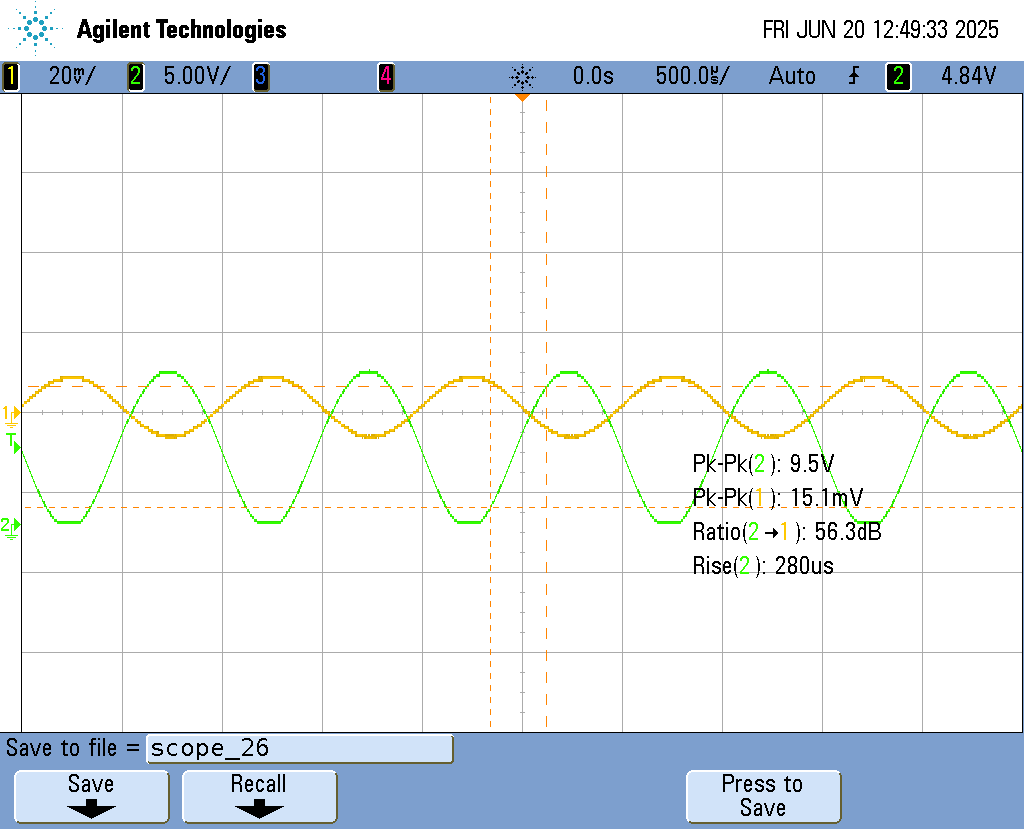
\includegraphics[width=0.8\textwidth]{Figures/scope_26.png}
	\caption{Unten Abgeflachtes Ausgangssignal.}
	\label{fig:supplyrailsmid}
\end{figure}
\begin{figure}[H]
	\centering
	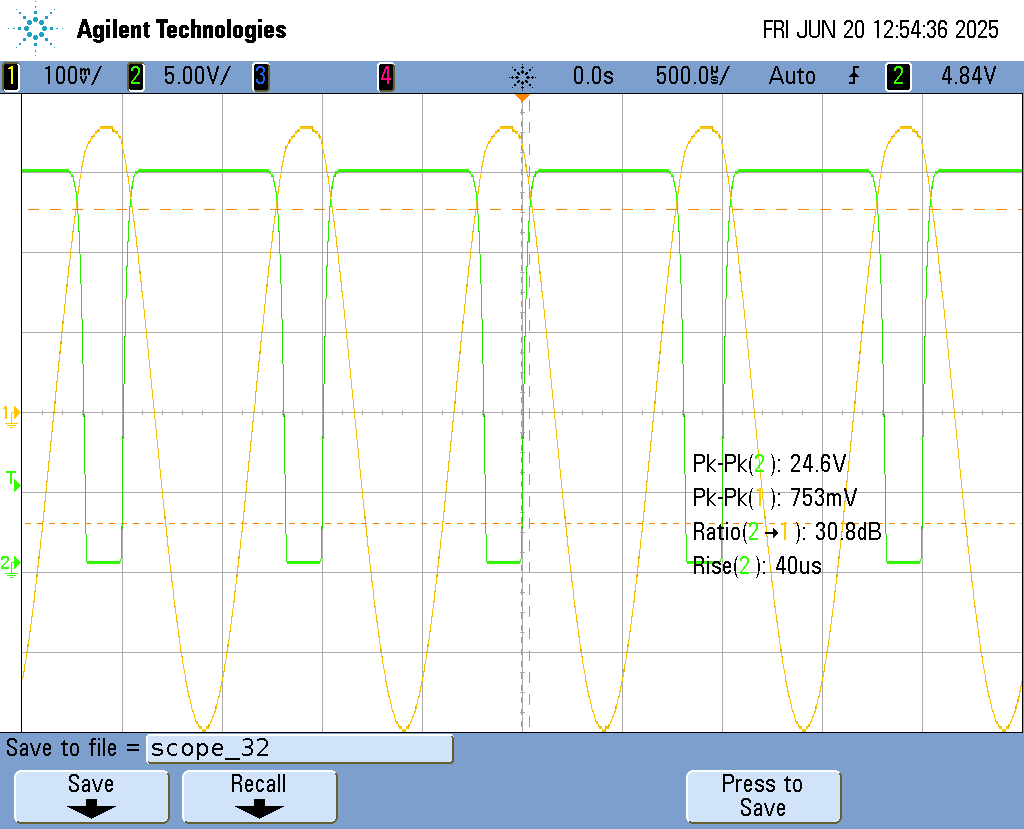
\includegraphics[width=0.8\textwidth]{Figures/supplyrailskrass.png}
	\caption{Abgeschnittenes Ausgangssignal.}
	\label{fig:supplyrailskrass}
\end{figure}

%scope_26.png
% B.2.3.
\subsubsection{Bandbreite}
Die untere Grenzfrequenz $f_{gu} = \SI{36.6}{\hertz}$ und die obere Grenzfrequenz $f_{go} = \SI{728}{\kilo\hertz}$ bestimmen die Bandbreite des Verstärkers. Die Bandbreite $B$ ergibt sich zu:
Dabei ist $f_{gu}$ die Frequenz, bei der die Verstärkung auf $\frac{1}{\sqrt{2}} \hat{=}\SI{-3}{\decibel}$ ihres Maximalwertes im unteren Frequenzbereich abfällt, und $f_{go}$ entsprechend im oberen Frequenzbereich.
Die Spannungsverstärkung leigt ca. bei $\SI{41.1}{\decibel}$. Die Grenzfrequenzen $f_{go}$ und $f_{go}$ liegen dann bei etwa $\SI{41.1}{\decibel} - \SI{3}{\decibel} = \SI{38.1}{\decibel}$.

\[
B = f_{go} - f_{gu} \approx \SI{728}{\kilo\hertz}
\]

% B.3.
\subsection{Schaltanwendung}
% B.3.1.
\subsubsection{Grundlagen}
\begin{figure}[H]
	\centering
	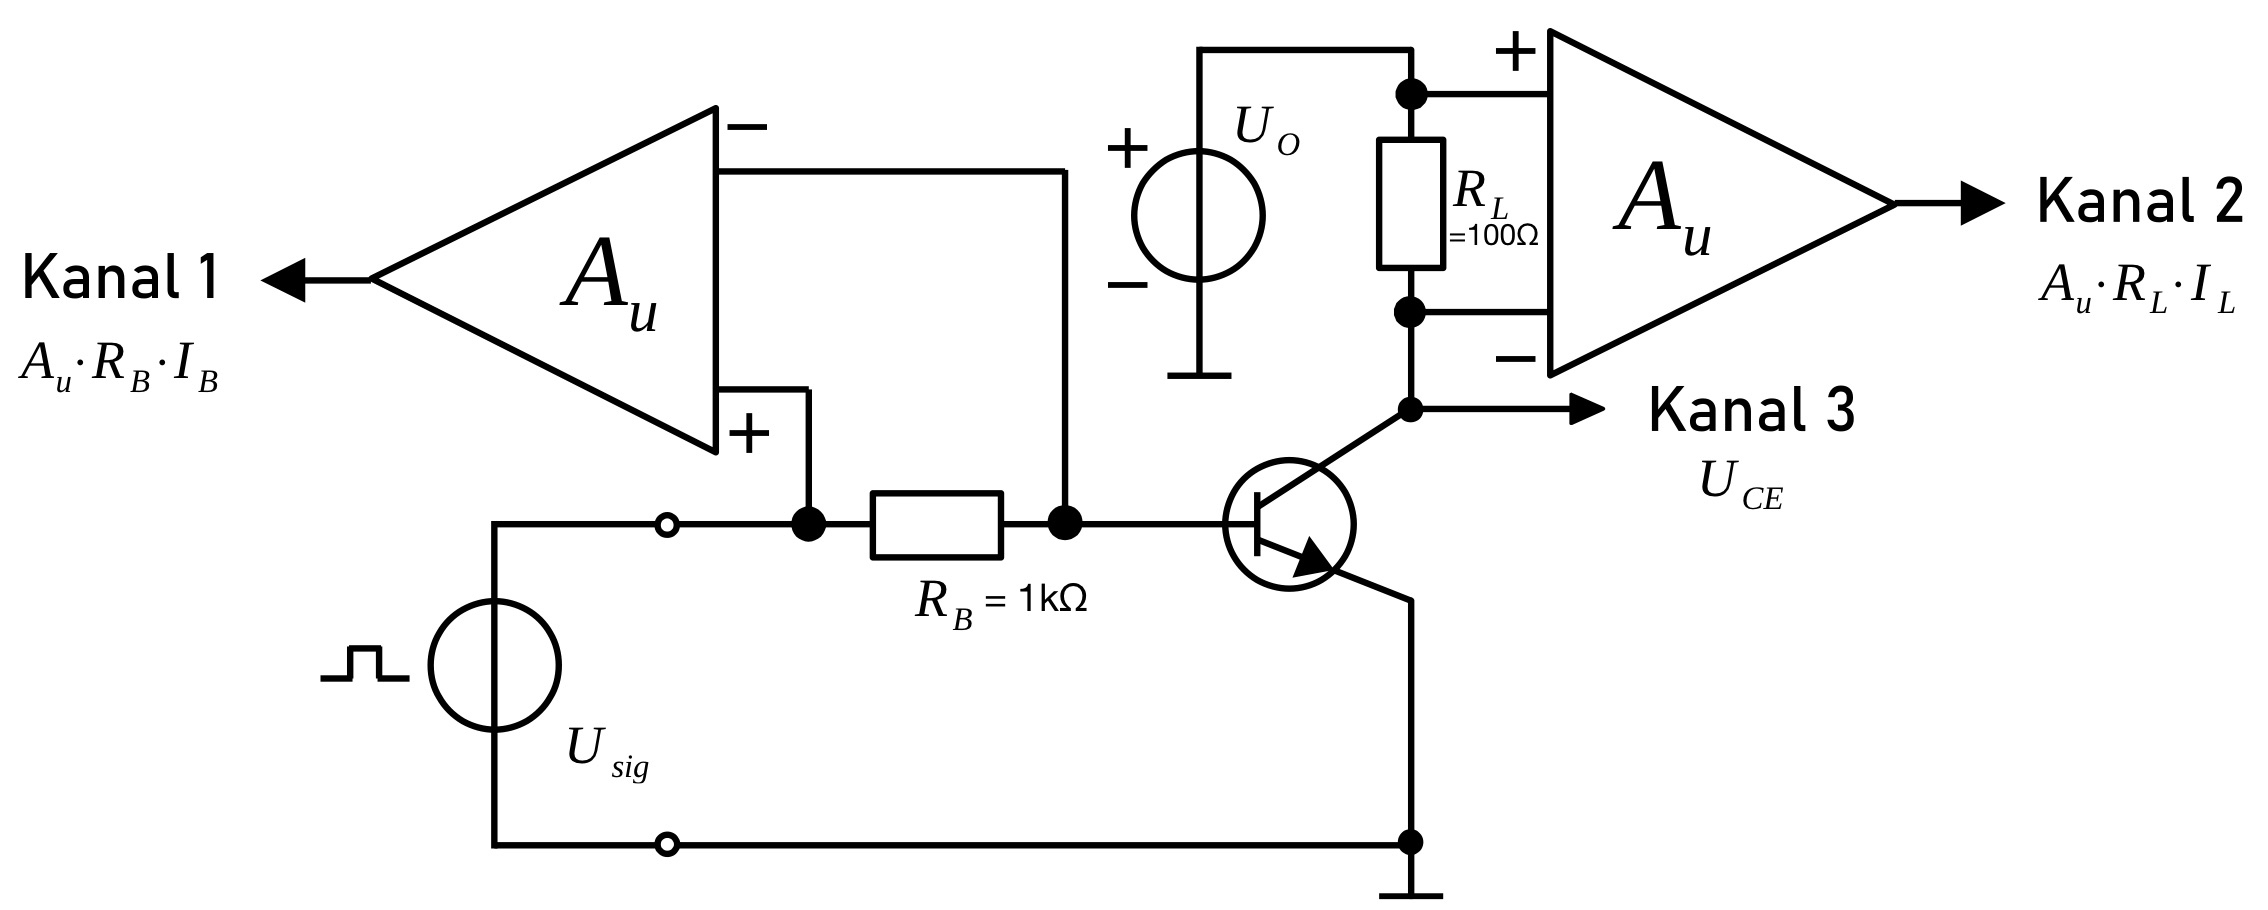
\includegraphics[width=0.7\textwidth]{Figures/MessschaltungSchaltanwendung.png}
	\caption{Messschaltung für Charakterisierung des Transistor als Schalter.}
	\label{fig:MessschaltungSchaltanwendung}
\end{figure}
Da bei der Versuchsdurchführung aus ungeklärten Gründen die Messung mit dem Oszilloskop nicht erfolgreich war, wird dieser Versuch mit LTSpice Simuliert. Dafür wird ein 2N3055 verwendet, welcher ähnliche Eigenschaften wie der Bipolartransistor im Labor vorweist.  
Der Basisstrom wird allerdings über eine Ideale Stromquelle festgelegt, jedoch mit gleichen Zeitlichen Parametern wie in der Versuchsanleitung.
Die Basisströme wurden mit ´´.step´´ alle in einem Diagramm Dargestellt. Dabei ist $I_B = \SI{300}{\micro\ampere}$ grün, $I_B = \SI{400}{\micro\ampere}$ blau, $I_B = \SI{500}{\micro\ampere}$ rot und $I_B = \SI{300}{\micro\ampere}$ türkis.
\begin{figure}[H]
	\centering
	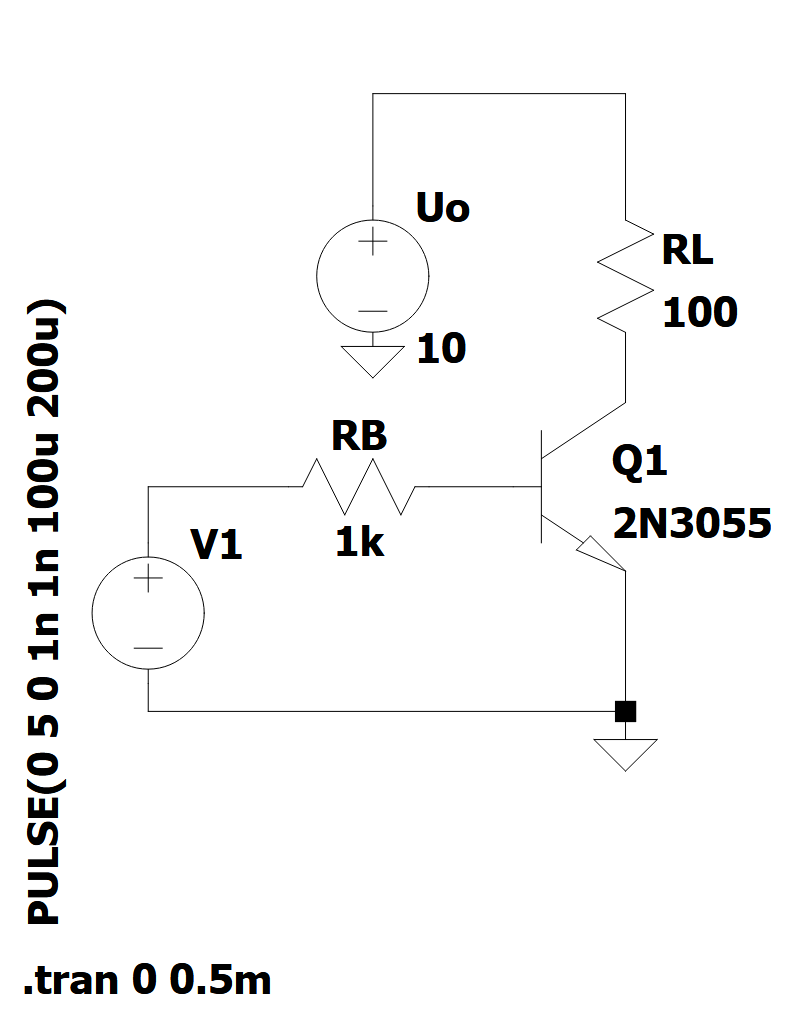
\includegraphics[width=0.7\textwidth]{Figures/LTSpiceSchaltung.png}
	\caption{Simulationsschaltung in LTSpice.}
	\label{fig:LTSpiceSchaltung}
\end{figure}

\begin{figure}[H]
	\centering
	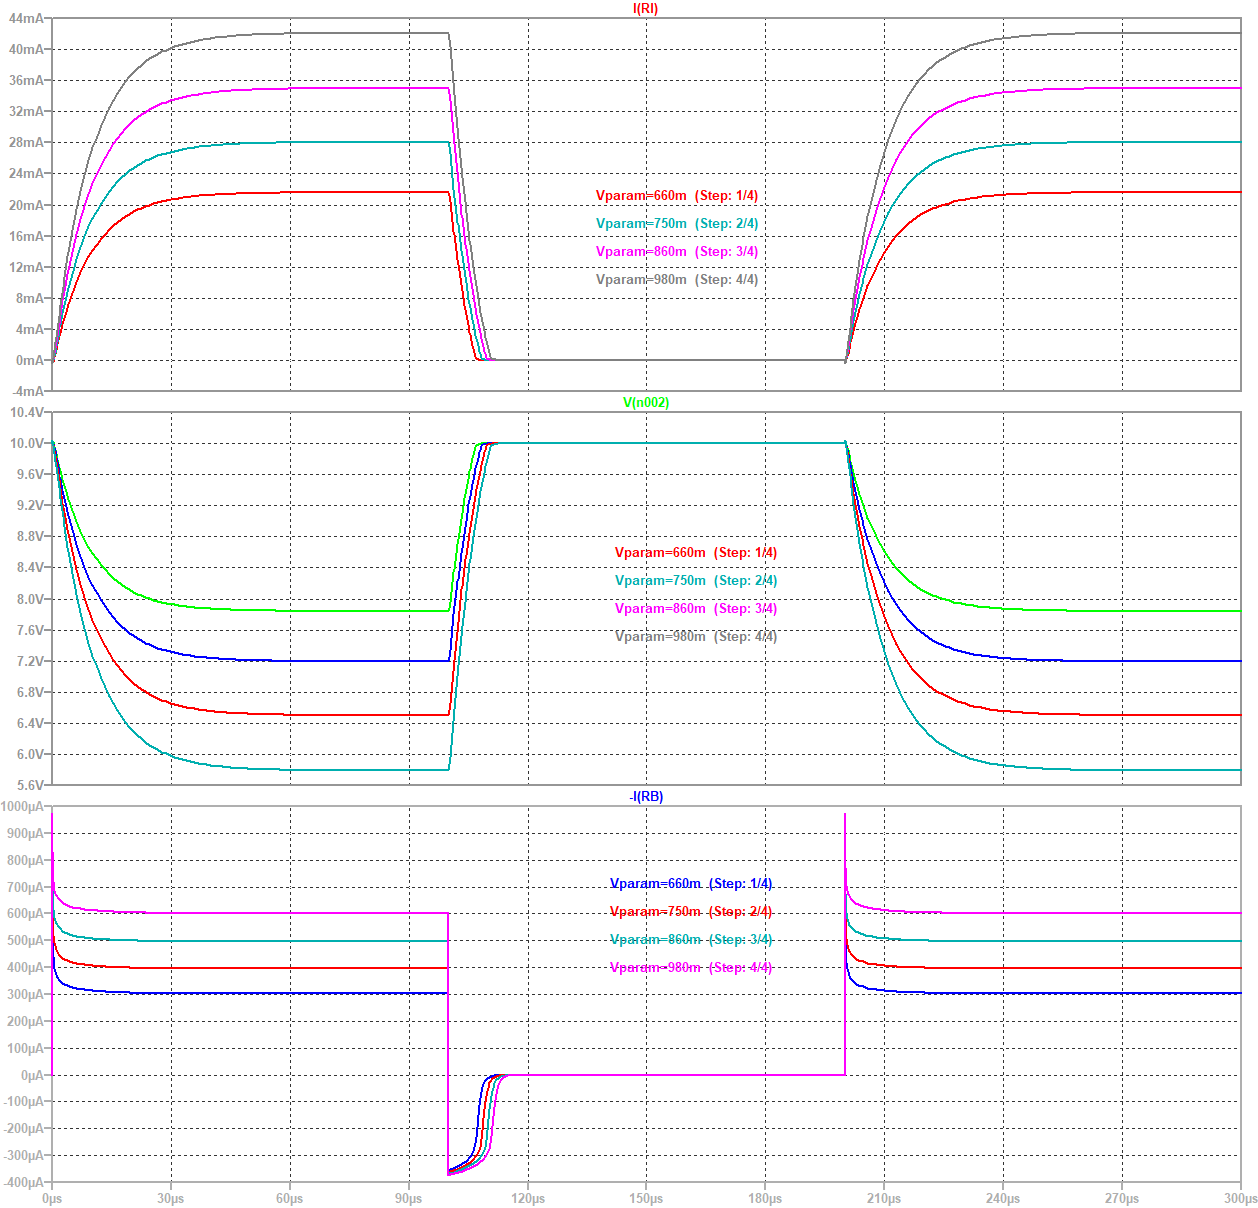
\includegraphics[width=0.9\textwidth]{Figures/LTSpiceTime300u.png}
	\caption{Zeitlicher Verlauf von $I_B$ (oben), $I_C$ (mitte), $U_{CE}$ (unten)}
	\label{fig:300uVerlauf3}
\end{figure}


\subsubsection{Ausschaltzeiten}

\subsubsection{Einschaltzeiten}

% C.
\section{Auswertung}
% C.1.1.
\subsection{Parameter}
\subsubsection{Ausgangskennlinienfeld}


\vspace{1em}
*** BILD MIT RESTLICHEN WERTEN EINFÜGEN ***
% Ausgangskennlinie für C.3.1 a
\begin{figure}[H]
	\centering
	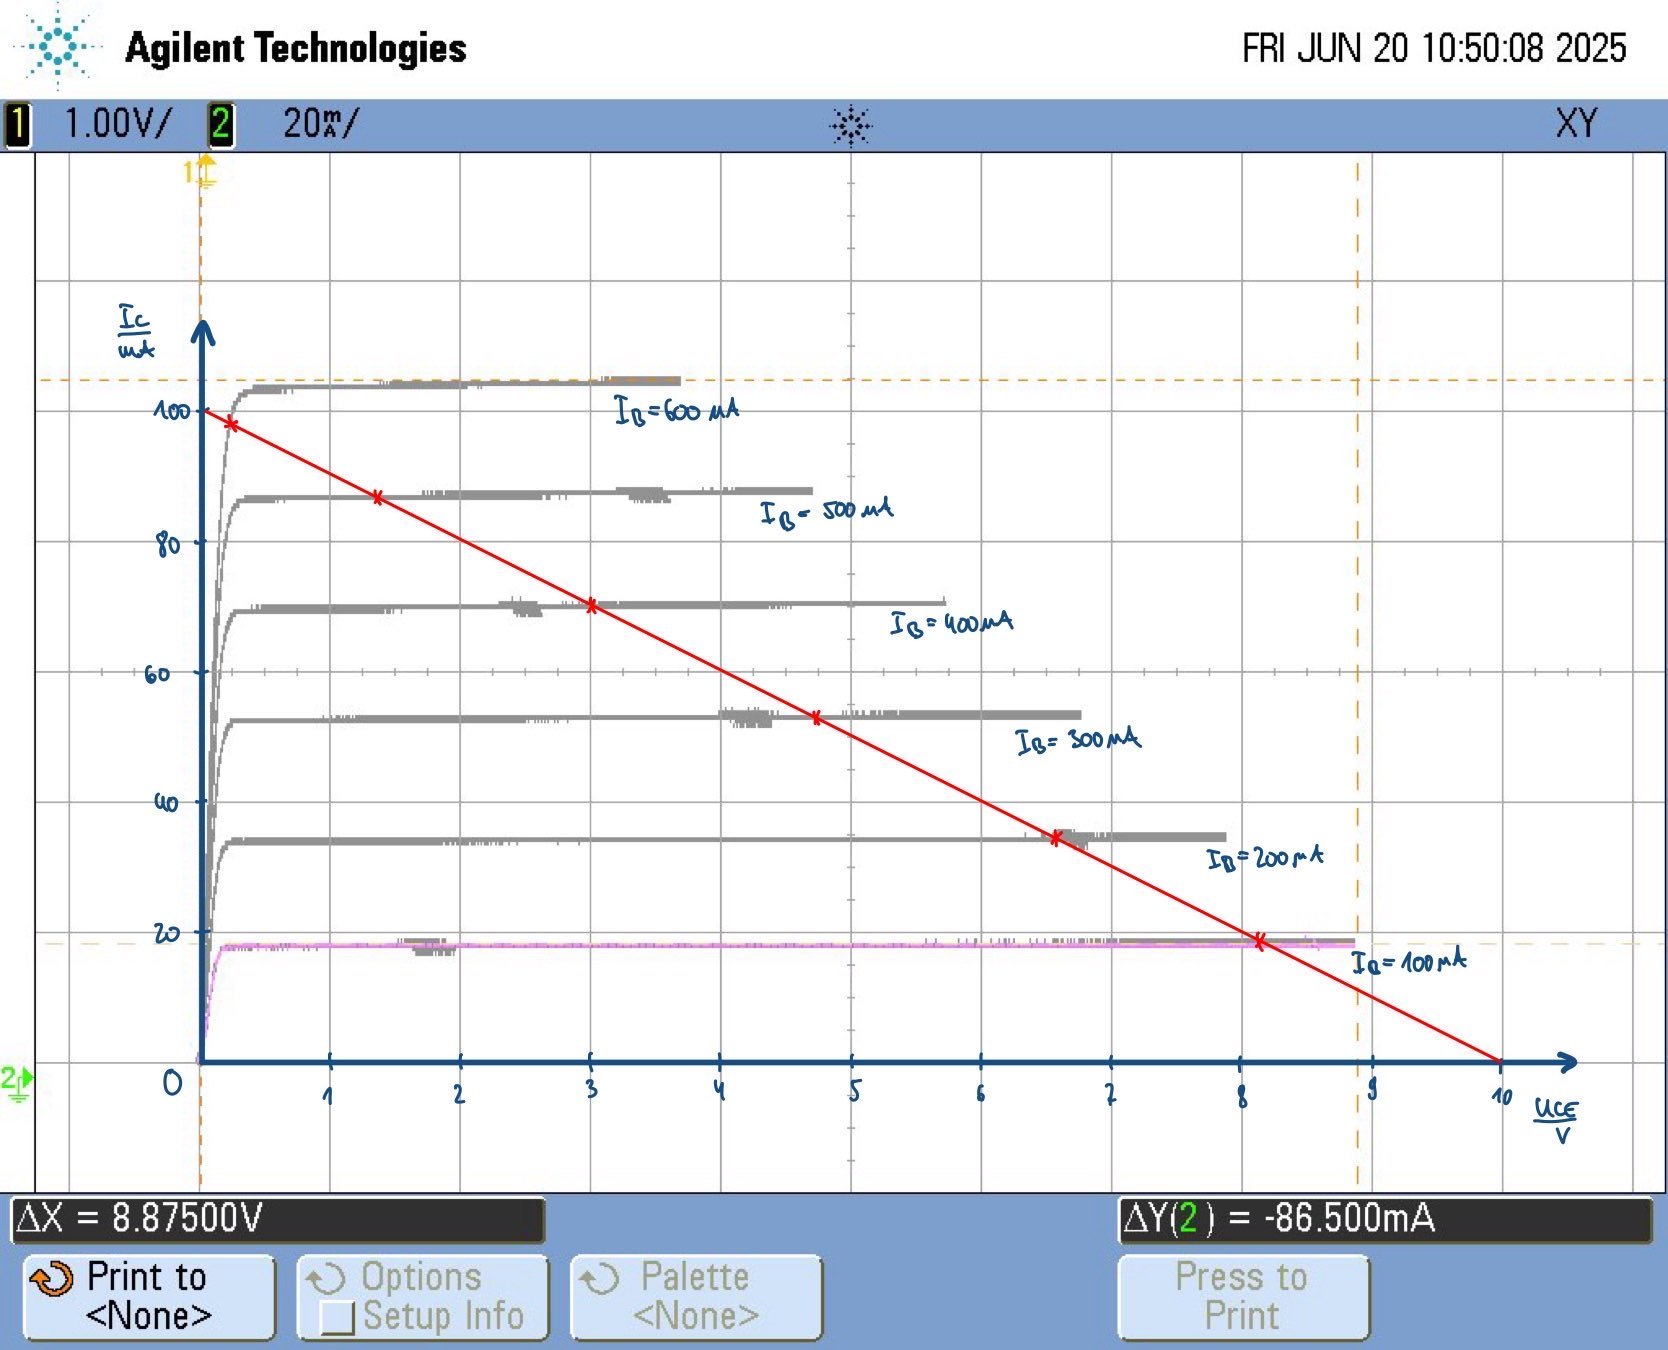
\includegraphics[width=0.8\textwidth]{Figures/scope_4_eingangskennlinie_C.3.1..jpg}
	\caption{Bestimmung der Arbeitspunkte des Transistors in Schaltkonfiguration.}
	\label{fig:arbeitspunkte schaltkonfiguration}
\end{figure}

\paragraph{a)}
Der hier sichtbare Widerstand ist durch die Wiederstände in Reihe mit dem Kollektor zurückzuführen. Die kürzeren Kennlinien bei höheren Basisströmen, liegt an dem geringeren Spannungsabfall $U_{CE}$, welche jetzt an $R_C + R_{gen}$ abfällt. 
\[
R_{\text{ges}} = R_{\text{gen}} + R_{\text{Leitung}} = \frac{\Delta U_{CE}}{\Delta I_C} = \frac{4\,\mathrm{V}}{65\,\mathrm{mA}} \approx 61.54\,\Omega
\]

wobei $\Delta U_{CE}$ die Spannungsänderung und $\Delta I_C$ die Stromänderung im betrachteten Bereich ist.


\paragraph{b)}

Die statische Stromverstärkung $B$ (auch $\beta$ genannt) berechnet sich zu $B = \frac{I_C}{I_B}$. Für jeden Messpunkt bei $U_{CE} = 5\,\mathrm{V}$ wird $I_C$ durch den zugehörigen $I_B$ geteilt und der Verlauf von $B$ über $I_B$ bzw. $I_C$ aufgetragen.
\begin{table}[H]
\centering
\begin{tabular}{c|c|c|c|c|c}
$I_{C}$ & 0mA   & 18.5mA   & 36mA    & 51mA    & 71mA    \\ \hline
$I_{B}$ & 0µA & 100µA & 200µA & 300µA & 400µA \\ \hline
$\beta_{IC/IB}$ & 0   & 185   & 180    & 170    & 177.5   
\end{tabular}
\caption{Stromverstärkung }
\label{tab:my-table}
\end{table}
\paragraph{c)}

Die gemessene Stromverstärkung $B$ liegt im Bereich des im Datenblatt angegebenen Wertes (hier $100 \sim 250$). Abweichungen sind vermutlich durch Messfehler oder Bauteiltoleranzen entstanden.

\paragraph{d)}

Die Early-Spannung $U_A$ ergibt sich als Schnittpunkt der verlängerten Kennlinie mit der $U_{CE}$-Achse. Dazu wird die Gerade durch die Kennlinie extrapoliert und der Schnittpunkt mit $I_C = 0$ bestimmt.
\[
U_A = I_0 \cdot \frac{\Delta U}{\Delta I} + U_{BE}= \frac{105\,\mathrm{mA} \cdot 9\,\mathrm{V}}{5\,\mathrm{mA}} + 720\,\mathrm{mV}= 189{,}72\,\mathrm{V}
\]
\paragraph{e)}

Die Übersteuerungsgrenze ist die Linie im Ausgangskennlinienfeld, für welche $U_{CB} = \SI{0}{V}$, also $U_{CE} = U_{BE}$ gilt. Links dieser Linie Grenze liegt der Sättigungsbereich.


% C.1.2.
\subsubsection{Eingangskennlinie}

Nun soll für einen Basisstrom von $600\,\mu\text{A}$ der Eingangswiderstand bestimmt werden.



In Abbildung \ref{fig:Eingangskennlinie} wurden bei $I_{B}$ folgende Werte für $\Delta U_{BE}$ und $\Delta I_B$ extrapoliert:

\[
\begin{aligned}
I_B = 600\,\mu\text{A}, \quad \Delta U_{BE} \approx 50\,\text{mV}, \quad \Delta I_B \approx 750\,\mu\text{A} \\
\end{aligned}
\]

\vspace{1em}

Somit erhalten wir für $r_{BE}$:

\[
\begin{aligned}
r_{BE} = \frac{\Delta U_{BE}}{\Delta I_B} = \frac{50\,\text{mV}}{750\,\mu\text{A}} = 66{,}67\,\Omega
\end{aligned}
\]

\subsubsection{Temperaturverhalten}
\paragraph{a)}
Aufgrund der Hysteresekurve bei $U_{CE} = \SI{8}{\volt}$ im Vergleich zu $U_{CE} = \SI{2}{\volt}$ lässt sich eine deutlich höhere Temperatur bei höherer Spannung vermuten. 
Bei $U_{CE} = \SI{8}{\volt}$ lässt sich zwischen $f = \SI{0.1}{\hertz}$ und $f = \SI{1}{\kilo\hertz}$ einen Unterschied in der Hysteresekurve erkennen. Diese ist bei der niedrigeren Frequenz viel Stärker ausgeprägt.  
Die erhöhte Temperatur hat tendenziell ein Verschieben der Eingangskennlinie nach links zur Folge, etwa $\frac{\SI{2}{\milli\volt}}{\SI{}{\kelvin}}$. 
Mit Abbildung \ref{fig:2V1eingang} und Abbildung \ref{fig:8V1khz0.1hzzusammentemp} lässt sich $\Delta U_{BE}$ zu $\SI{710}{\milli\volt} - \SI{660}{\milli\volt} = \SI{60}{\milli\volt}$ bestimmen.
\[
\Delta T = \frac{\Delta U}{\frac{\SI{2}{\milli\volt}}{\SI{}{\kelvin}}} = \SI{30}{\kelvin}
\]
\paragraph{b)}

Der in a) angenommene Temperaturunterschied muss zur Raumtemperatur addiert werden, um die Chiptemperatur zu bestimmen: $\Delta T + \SI{23}{\degreeCelsius} = \SI{53}{\degreeCelsius}$.\\
Die Abkühlrate kann mit hilfe der Kennlinie in Abbildung \ref{fig:8VTemperaturHysterese0.1hznah} bestimmt werden.
Da die Frequenz bei hoher Hysterese $\SI{0.1}{\hertz}$ beträgt, führt dies auf eine Abkühldauer von $\SI{5}{\second}$.\\

\[
\Delta U_{BE,H} = \SI{12.5}{\milli\volt} \rightarrow \Delta T = \frac{\Delta U_{BE,H}}{\frac{\SI{2}{\milli\volt}}{\SI{}{\kelvin}}} = \SI{6.25}{\kelvin}
\rightarrow \frac{\Delta T}{\SI{5}{\second}} = \SI{1.25}{\kelvin\per\second}
\]
%
%Das Temperaturverhalten des Transistor lässt sich mithilfe des Datenblatt bestimmen. 
%\[
%\Delta T = P \cdot R_{th,C} \hspace{1cm} P_{Transistor} = U_{CE} \cdot I_{B} \cdot \beta \hspace{1cm} R_{th,C} = \SI{10}{\degreeCelsius\per\watt} \hspace{1cm} \beta \approx 200
%\]
%\[
%P_{\SI{8}{\volt}} = \SI{8}{\volt} \cdot \SI{1}{\milli\ampere} \cdot 200 = \SI{1.6}{\watt} \hspace{1cm} P_{\SI{2}{\volt}} = \SI{2}{\volt} \cdot \SI{1}{\milli\ampere} \cdot 200 = \SI{0.8}{\watt}
%\]
%\[
%\Delta T_{\SI{8}{\volt}} = \SI{1.6}{\watt} \cdot \SI{10}{\degreeCelsius\per\watt} = \SI{16}{\kelvin} \hspace{1cm} \Delta T_{\SI{8}{\volt}} = \SI{0.8}{\watt} \cdot \SI{10}{\degreeCelsius\per\watt} = \SI{8}{\kelvin}
%]


\subsubsection{Übertragunskennlinie}
\begin{figure}[H]
	\centering
	\includegraphics[width=0.8\textwidth]{Figures/Übertragungskennlinie.png}
	\caption{Übertragungskennlinie.}
	\label{fig:Übertragungskennlinie}
\end{figure}

Die Berechnung der realen sowie theoretischen Steilheit ergibt:\\

\[
g_m \approx \frac{\Delta I_C}{\Delta U_{BE}} = \frac{\SI{32.5}{\milli\ampere}}{\SI{48}{\milli\volt}} \approx \SI{0.677}{\siemens}
\]
\[
g_{\text{m, theoretisch}} = \frac{I_{\text{C}}}{U_{\text{T}}} = \frac{20\,\text{mA}}{25,8\,\text{mV}} = 0.775194\,\text{S}
\]

\vspace{2em}
Die ermittelten Werte stimmen im Rahmen der Messungenauigkeit mit den theoretischen überein.

\subsection{Verstärker}
\paragraph{a)}

Die lineare Quellkennlinie beschreibt den Zusammenhang zwischen Kollektorstrom $I_C$ und Kollektor-Emitter-Spannung $U_{CE}$ für einen gegebenen Arbeitswiderstand $R_C$ und eine Versorgungsspannung $U_{o2}$:

\[
I_C(U_{CE}) = \frac{U_{o2} - U_{CE}}{R_C}
\]

Für $U_{CE} = \SI{0}{\volt}$ ergibt sich:

\[
I_C(\SI{0}{\volt}) = \frac{\SI{20}{\volt}}{\SI{1}{\kilo\ohm}} = \SI{20}{\milli\ampere}
\]

Für $U_{CE} = \SI{10}{\volt}$ ergibt sich:

\[
I_C(10\,\mathrm{V}) = \frac{\SI{20}{\volt}- \SI{10}{\volt}}{\SI{1}{\kilo\ohm}} = \SI{10}{\milli\ampere}
\]

\vspace{1em}
Die Arbeitsgerade verläuft also von $(U_{CE}, I_C) = (\SI{0}{\volt}, \SI{20}{\milli\ampere})$ durch $(\SI{10}{\volt}, \SI{10}{\milli\ampere})$.

\paragraph{b)}
Bei zu großen Eingangsamplituden verlässt der Transistor den linearen Arbeitsbereich. Das Ausgangssignal wird dann an den Versorgungsspannungen begrenzt, sodass die Signalform verzerrt wird (siehe Abbildung~\ref{fig:supplyrailskrass}).\\
Bereits bei geringeren Amplituden kann es durch die nichtlineare Eingangskennlinie (Abbildung~\ref{fig:Eingangskennlinie}) zu Verzerrungen kommen. Die maximale unverzerrte Ausgangsamplitude hängt daher sowohl von der Versorgungsspannung als auch von der Steilheit der $I_B(U_{BE})$-Kennlinie im Arbeitspunkt ab.\\ 
Für Spannungen des Eingangssignal unterhalb dessen Mittelwert ist eine Abflachung des Verstärkten Signal früher zu erkennen, weil der Transistor für diese Spannungen im Sättigungsbereich arbeitet. Deshalb ist der Schnitt unten am verstärkten Signal eher Abgerundet. 

\paragraph{c)}
Die Spannungsverstärkung $v_u$ berechnet sich als Verhältnis der Ausgangs- zur Eingangsamplitude:
\[
v_u = \frac{u_{pp-{Ausgang}}}{u_{pp-{Eingang}}}
\]
\begin{table}[H]
\centering
\begin{tabular}{c|c|c|c|c|c}
$I_C$                  & 2mA                     & 5mA                & 10mA               & 15mA               & 20mA               \\ \hline
$\hat{u}_{pp-Eingang}$ &
  $\SI{9.9}{\milli\volt}$ &
  $\SI{9.7}{\milli\volt}$ &
  $\SI{9.3}{\milli\volt}$ &
  $\SI{8.9}{\milli\volt}$ &
  $\SI{8.6}{\milli\volt}$ \\ \hline
$\hat{u}_{pp-Ausgang}$ & $\SI{749}{\milli\volt}$ & $\SI{1.75}{\volt}$ & $\SI{3.25}{\volt}$ & $\SI{4.45}{\volt}$ & $\SI{5.53}{\volt}$ \\ \hline
\multicolumn{1}{l|}{$v_u$} &
  \multicolumn{1}{l|}{$75.7$} &
  \multicolumn{1}{l|}{$180.4$} &
  \multicolumn{1}{l|}{$349.5$} &
  \multicolumn{1}{l|}{$500.0$} &
  \multicolumn{1}{l}{$643.0$}
\end{tabular}
\caption{Aus und Eingangsamplituden bei Verschiedenen Kollektorströmen.}
\label{spannungsverstrkung}
\end{table}
\begin{figure}[H]
	\centering
	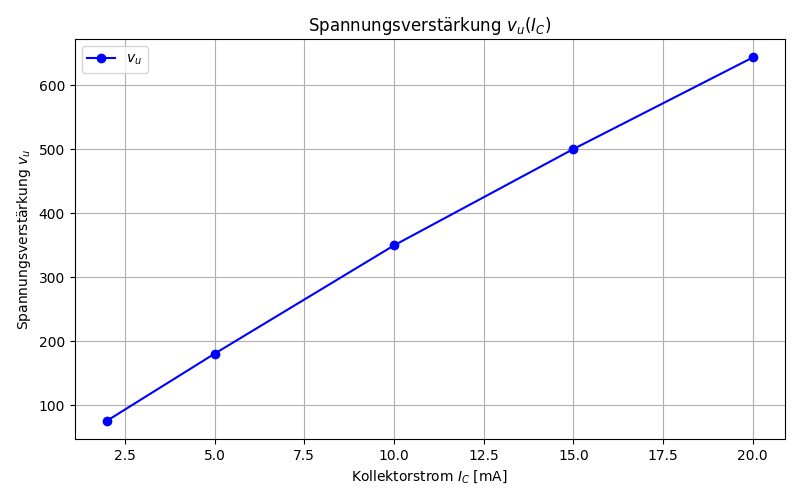
\includegraphics[width=0.9\textwidth]{Figures/vuplot.png}
	\caption{Spannungsverstärkung über Kollektorstrom.}
	\label{fig:vuplot}
\end{figure}


\paragraph{d)}

Die Berechnung der Spannungsverstärkung ergibt:\\

\[
r_{CE} \approx \frac{U_A}{|I_C|} = \frac{\SI{189.72}{\volt}}{\SI{20}{\milli\ampere}} = \SI{9486}{\ohm} \\ 
\]
\[
v_u = g_m \cdot (r_{CE} \parallel R_C) \approx \SI{612.5}{}
\]

\vspace{1em}
Die berechneten Werte für \( I_C = \SI{20}{\milli\ampere} \) stimmt gut mit der gemessenen Spannungsverstärkung in diesem Arbeitspunkt überein. Unter Berücksichtigung von Messungenauigkeiten, Ablesefehlern bei der Bestimmung der Early-Spannung sowie der verwendeten Näherung für \( R_{CE} \) liegt das Ergebnis im erwarteten Rahmen. Diese Faktoren führen zu gewissen Ungenauigkeiten, beeinflussen das Gesamtergebnis jedoch nur geringfügig.



\subsection{Schalter}
\subsubsection{Arbeitspunkte}

\paragraph{a)}

Um die verschiedenen Arbeitspunkte zu bestimmen wurde eine Arbeitsgerade in das Ausgangskennlinienfeld gelegt. Die beiden Punkte hierfür erhält man indem man den Transistor im Sperr- und Sättigungsbereich betrachtet:

\begin{align*}
\text{Punkt 1:} \quad & I_C = 0 \Rightarrow U_{CE} = U_{02} = 10\,\text{V} \\
\text{Punkt 2:} \quad & U_{CE} = 0 \,\, (\text{da Kurzschluss}) \Rightarrow I_C = \frac{10\,\text{V}}{100\,\Omega} = 100\,\text{mA}
\end{align*}

\vspace{1em}

Anschleißend wurden folgende Werte entnommen (siehe Abbildung~\ref{fig:arbeitspunkte schaltkonfiguration}):

\begin{table}[H]
\centering
\begin{tabular}{c|c|c|c|c}
$I_B$ (µA) & $U_{CE}$ (in V) & $U_{CE}$ (in V) & $I_C$ (in mA) & $\beta = \frac{I_C}{I_B}$ \\ \hline
600 & 0,2 & **vergleichswerte** &  &  \\ \hline
500 & 1,35 &  &  &  \\ \hline
400 & 3,0 &  &  &  \\ \hline
300 & 4,8 &  &  &  **vergleichswerte**
\end{tabular}
\caption{Auswertung der Arbeitspunkte bei verschiedenen Basisströmen}
\label{tab:arbeitspunkte}
\end{table}


Die gemessenen Werte stimmen im Rahmen der Zeichen- und Messgenauigkeit überein.

\paragraph{b)}
*** ACHTUNG RECHNUNG MIT PROVISORISCHEN WERTEN, MÜSSEN NOCH AUSGEBESSERT WERDEN***\\

Ideale Schalterleistung:

\[
P_L = \frac{U_0^2}{R_L} = \frac{(10\,\text{V})^2}{100\,\Omega} = 1\,\text{W}
\]

Transistor als Schalter:

\[
P_L = \frac{(U_0 - U_{CE})^2}{R_L}
\]
\vspace{1em}
\[
P_{(I_B = 0{,}6\,\text{mA})} = \frac{(10\,\text{V} - 192{,}59\,\text{mV})^2}{100\,\Omega} = 96{,}785\,\text{mW}
\]
\vspace{1em}
\[
\rightarrow P_{(I_B = 0{,}5\,\text{mA})} = 725{,}65\,\text{mW}
\]
\[
\rightarrow P_{(I_B = 0{,}4\,\text{mA})} = 474{,}57\,\text{mW}
\]

\vspace{1em}

Für ein steigendes $I_B$ wird der Transistor somit immer mehr zu einem idealen Schalter.


\subsubsection{Schaltzeiten}


\paragraph{a)}

Die Speicherzeit \( t_s \) ergibt sich aus:

\begin{equation}
t_s = \Delta t = \frac{\Delta Q_D}{I_{RM}}
\end{equation}

\begin{table}[H]
\centering
\begin{tabular}{c|c}
\textbf{\( I_B \) (µA)} & \textbf{\( t_s \) (ns)} \\
\hline
600 &  \\
\hline
500 &  \\
\hline
400 &  \\
\hline
300 &  \\
\end{tabular}
\caption{Speicherzeiten bei verschiedenen Basisströmen}
\label{tab:Schaltzeiten}
\end{table}




\paragraph{b)}

Wir messen Ein- und Ausschaltzeiten im Bereich von \( 0{,}1 \cdot I_C \) bis \( 0{,}9 \cdot I_C \).


Die Einschaltzeiten  \( t_e \) ergeben sich aus:

\begin{table}[H]
\centering
\begin{tabular}{c|c}
\textbf{\( I_B \) (µA)} & \textbf{\( t_e \) (ms)} \\
\hline
600 &  \\
\hline
500 &  \\
\hline
400 &  \\
\hline
300 &  \\
\end{tabular}
\caption{Einschaltzeiten bei verschiedenen Basisströmen}
\label{tab:Schaltzeiten}
\end{table}


Die Ausschaltzeiten  \( t_a \) ergeben sich aus:

\begin{table}[H]
\centering
\begin{tabular}{c|c}
\textbf{\( I_B \) (µA)} & \textbf{\( t_a \) (ns)} \\
\hline
600 &  \\
\hline
500 &  \\
\hline
400 &  \\
\hline
300 &  \\
\end{tabular}
\caption{Ausschaltzeiten bei verschiedenen Basisströmen}
\label{tab:Schaltzeiten}
\end{table}




%\printbibliography % Output the bibliography

%----------------------------------------------------------------------------------------
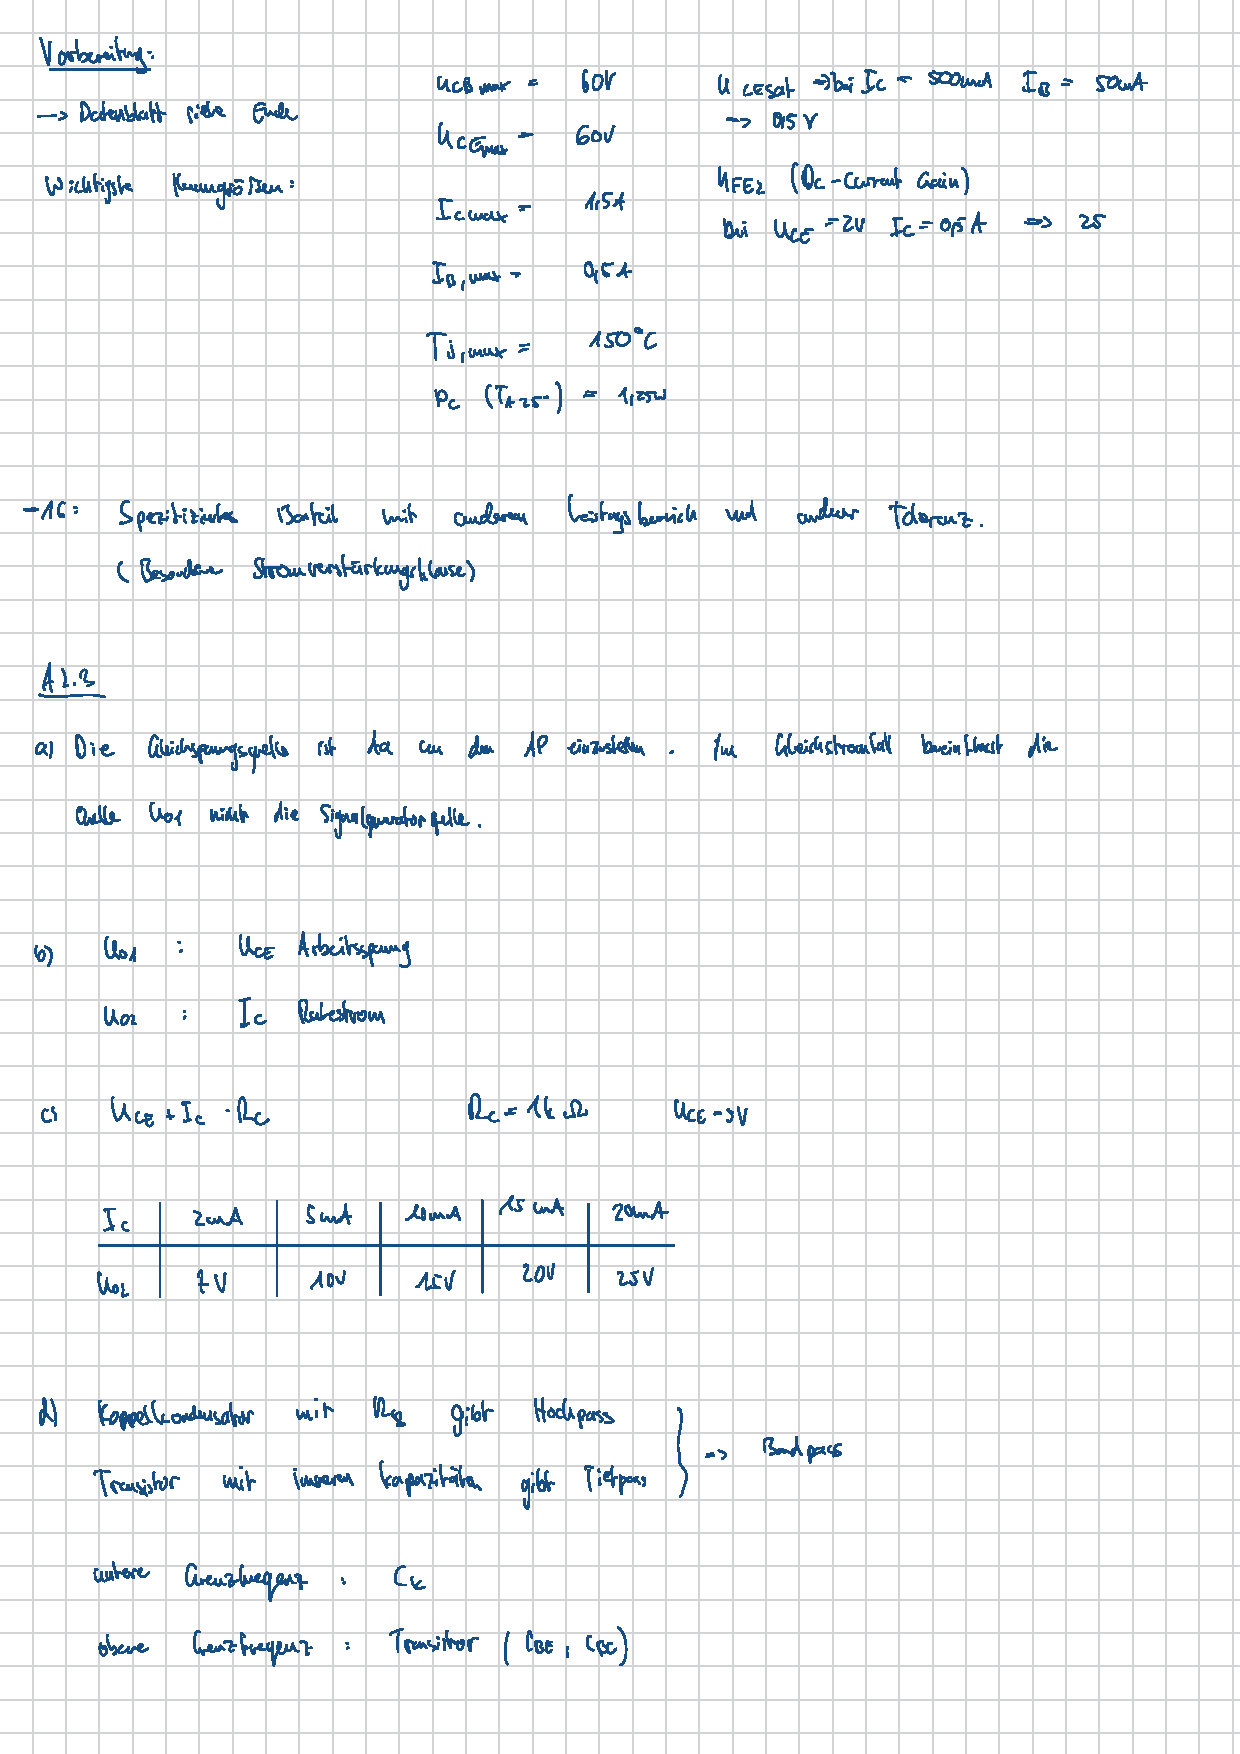
\includepdf[pages={1}]{Vorbereitung.pdf}

\end{document}